\Section{Move Prover Design}

\begin{Figure}
  \centering
  \caption{Move Prover Architecture}
  \label{fig:Arch}
  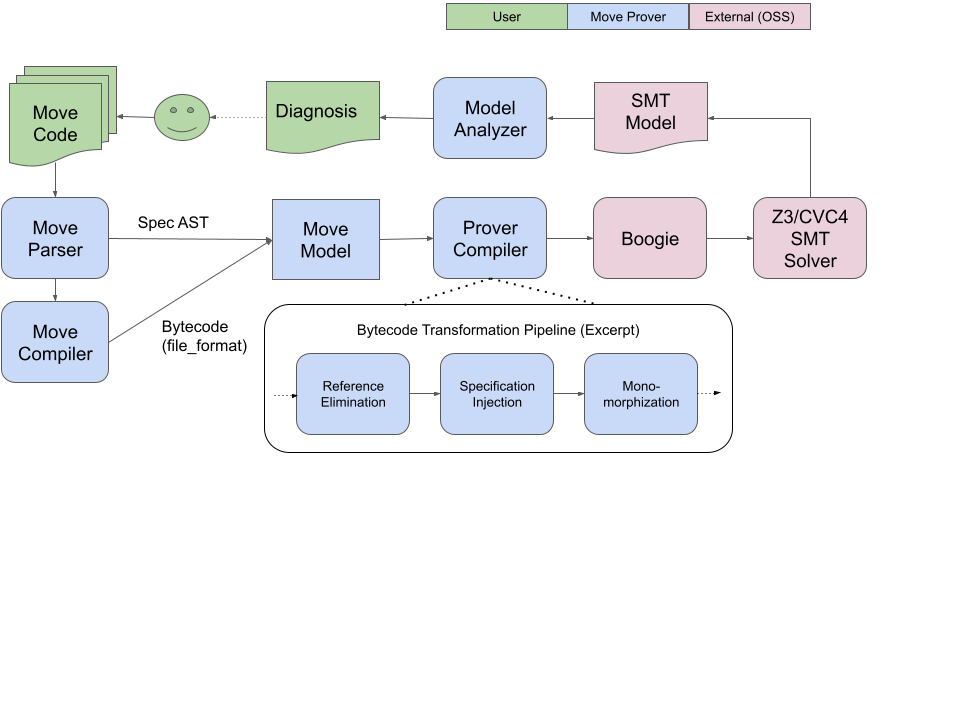
\includegraphics[trim=0 250 0 0, width=\textwidth]{arch.png}
\end{Figure}

The architecture of \MVP is illustrated in Fig.~\ref{fig:Arch}. Move code
(containing specifications) is given as input to the Move tool chain, which
produces two artifacts: the abstract syntax tree (AST) of the specifications,
and the generated bytecode.  The \emph{Move Model} merges both bytecode and
specifications, as well as other metadata from the original code, into a unique
object model which is input to the remaining tool chain.

The next phase is the actual \emph{Prover Compiler}, which is implemented as a
pipeline of bytecode transformations. Only an excerpt of the most important
transformations is shown (Reference Elimination, Specification Injection, and
Monomorphization). These transformations will be conceptually described in more
detail in subsequent sections. While they happen in reality on an extended
version of the bytecode, we will illustrate them on a higher level of
abstraction, as Move source level transformations.

The transformed bytecode is next compiled into the Boogie intermediate
verification language \cite{BOOGIE}. Boogie supports an imperative programming
model which is well suited for the encoding of the transformed Move code. Boogie
in turn can translate to multiple SMT solver backends, namely Z3 \cite{Z3} and
CVC5 \cite{CVC}; the default choice for the Move prover is currently Z3.

% When the SMT solver produces a |sat| or |unknown| result (of the negation of the
% verification condition Boogie generates), it produces a model witness. The Move
% Prover attempts to translate this model back into a diagnostic which
% a user can associate with the original Move code (as has been illustrated in
% Sec.~\ref{sec:RunningProver}.) For example, execution traces leading to the
% verification failure are shown, with assignments to variables used in this
% trace, extracted from the model. Also the Move Model will be consulted to
% retrieve the original source information and display it with the diagnosis.

Subsequently, we will focus on the major bytecode transformations.

\SubSection{Reference Elimination}
\label{sec:RefElim}

The Move language supports references to data stored in global memory and on the
stack. Those references can point to interior parts of the data. The reference
system is based on \emph{borrow semantics} \cite{BORROW_SEM} as it is also found
in the Rust programming language.  One can create (immutable) references |&x|
and mutable references |&mut x|, and derive new references by field selection
(|&mut x.f| and |&x.f|). The borrow semantics of Move provides the following
guarantees (ensured by the borrow checker~\cite{BORROW_CHECKER}):

\begin{itemize}
\item For any given location in global memory or on the stack, there can be
  either exactly one mutable reference, or $n$ immutable references. Hereby,
  it does not matter to what interior part of the data is referred to.
\item Dangling references to locations on the stack cannot exist; that is, the
  lifetime of references to data on the stack is restricted to the lifetime of the
  stack location.
\end{itemize}

\noindent These properties enable us to \emph{effectively eliminate} references from the Move
program, reducing the verification complexity significantly, as we do not need to
reason about sharing. It comes as no surprise that the same discipline of borrowing
which makes Move (and Rust) programs safer by design also makes verification simpler.

\Paragraph{Immutable References}

Since during the existence of an immutable reference no mutation on the
referenced data can occur, we can simply replace references by the referred
value.

An example of the applied transformation is shown below. We remove the reference
type constructor and all reference-taking operations from the code:

\begin{Move}
  fun select_f(s: &S): &T { &s.f } @\transform@ fun select_f(s: S): T { s.f }
\end{Move}


\noindent Notice that at Move execution time, immutable references serve
performance and ownership objectives (avoid copies); however, the symbolic
reasoning engines we use have a different representation of values, in which
structure sharing is common and copying is cheap.

\Paragraph{Mutable References}
\label{sec:RefElimMut}

Each mutation of a location |l| starts with an initial borrow for the whole data
stored in this location (in Move, |borrow_global_mut<T>(addr)| for global
memory, and |&mut x| for a local on the stack). Let's call the reference
resulting from such a borrow |r|. As long as this reference is alive, Move code
can either update its value (|*r = v|), or derive a sub-reference~%
(|r' = &mut r.f|). The mutation ends when |r| (and the derived |r'|) go out of
scope.  Because of the guarantees of the borrow semantics, during the mutation
of the data in |l| no other reference can exist into data in |l|.

The fact that |&mut| has exclusive access to the whole value in a location
allows to reduce mutable references to a \emph{read-update-write} cycle. One can
create a copy of the data in |l| and single-thread it to a sequence of
mutation steps which are represented as purely functional data updates.  Once
the last reference for the data in |l| goes out of scope, the updated value is
written back to |l|. This effectively turns an imperative program with references
into an imperative program which only has state updates on global memory or
variables on the stack, a class of programs which is known to have a significantly
simpler semantics. We illustrate the basics of this approach by an example:

\begin{Move}
  fun increment(x: &mut u64) { *x = *x + 1 }
  fun increment_field(s: &mut S) { increment(&mut s.f) }
  fun caller(): S { let s = S{f:0}; update(&mut s); s }
  @\transform@
  fun increment(x: u64): u64 { x + 1 }
  fun increment_field(s: S): S { s[f = increment(s.f)] }
  fun caller(): S { let s = S{f:0}; s = update(s); s }
\end{Move}

\Paragraph{Dynamic Mutable References}

While the setup in above example covers a majority of the use cases in every day
Move code, there are more complex ones to consider, namely that the value of a
reference depends on runtime decisions. Consider the following Move code:

\begin{Move}
  let r = if (p) &mut s1 else &mut s2;
  increment_field(r);
\end{Move}

\noindent Additional information in the logical encoding is required to deal
with such cases. At the execution point a reference goes out of scope, we need
to know from which location it was derived, so we can write back the updated
value correctly. Fig.~\ref{fig:MutElim} illustrates the approach for doing
this. A new Move prover internal type |Mut<T>| is introduced which carries the
location from which |T| was derived together with the value. It supports the
following operations:

\begin{itemize}
\item |Mvp::mklocal(value, LOCAL_ID)| creates a new mutation value for a local
  with the given local id.  Local ids are transformation generated constants
  kept opaque here.
\item Similarly, |Mvp::mkglobal(value, TYPE_ID, addr)| creates a new
  mutation for a global with given type and address. Notice that in the
    current Move type system, we would not need to represent the address, since
    there can be only one mutable reference into the entire type (via the
    acquires mechanism). However, we keep this more general here, as the Move
    type system might change.
\item With |r' = Mvp::field(r, FIELD_ID)| a mutation value for a sub-reference is
  created for the identified field.
\item The value of a mutation is replaced with |r' = Mvp::set(r, v)| and
  retrieved with |v = Mvp::get(r)|.
\item With the predicate |Mvp::is_local(r, LOCAL_ID)| one can test whether |r|
  was derived from the given local, and with |Mvp::is_global(r, TYPE_ID, addr)|
  whether it was derived from the specified global.~%
  |Mvp::is_field(r, FIELD_ID)| tests whether it is derived from the given field.
\end{itemize}

\begin{figure}[t!]
  \caption{Elimination of Mutable References}
  \label{fig:MutElim}
  \centering
\begin{MoveBoxNumbered}
  fun increment(x: &mut u64) { *x = *x + 1 }
  fun increment_field(s: &mut S) {
    let r = if (s.f > 0) &mut s.f else &mut s.g;
    increment(r)
  }
  fun caller(p: bool): (S, S) {
    let s1 = S{f:0, g:0}; let s2 = S{f:1, g:1};
    let r = if (p) &mut s1 else &mut s2;
    increment_field(r);
    (s1, s2)
  }
  @\transform@
  fun increment(x: Mut<u64>): Mut<u64> { Mvp::set(x, Mvp::get(x) + 1) }
  fun increment_field(s: Mut<S>): Mut<S> {
    let r = if (s.f > 0) Mvp::field(s.f, S_F) else Mvp::field(s.g, S_G);
    r = increment(r);
    if (Mvp::is_field(r, S_F))
      s = Mvp::set(s, Mvp::get(s)[f = Mvp::get(r)]);
    if (Mvp::is_field(r, S_G))
      s = Mvp::set(s, Mvp::get(s)[g = Mvp::get(r)]);
    s
  }
  fun caller(p: bool): S {
    let s1 = S{f:0, g:0}; let s2 = S{f:1, g:1};
    let r = if (p) Mvp::mklocal(s1, CALLER_s1)
            else Mvp::mklocal(s2, CALLER_s2);
    r = increment_field(r);
    if (Mvp::is_local(r, CALLER_s1))
      s1 = Mvp::get(r); @\label{line:WriteBack}@
    if (Mvp::is_local(r, CALLER_s2))
      s2 = Mvp::get(r);
    (s1, s2)
  }
\end{MoveBoxNumbered}
\end{figure}

The Move Prover has a partial implementation of the illustrated transformation.
The completeness of this implementation has not yet been formally investigated,
but we believe that it covers all of Move, with the language's simplification
that we do not need to distinguish addresses in global memory
locations.\footnote{\TODO{wrwg}{Need to investigate loops!}} (See discussion of
|Mvp::mkglobal| above.) The transformation also relies on that in Move there are
no recursive data types, so field selection paths are statically known. While
those things can be potentially generalized, we have not yet investigated this
direction.

The implementation constructs a \emph{borrow graph} from the program via a data
flow analysis. The borrow graph tracks both when references are released as well
as how they relate to each other: e.g. |r' = &mut r.f| creates a edge from |r|
to |r'| labeled with |f|, and |r' = &mut r.g| creates another also starting
from |r|. For the matter of this problem, a reference is not released until a
direct or indirect borrow on it goes out of scope; notice that its lifetimes in
terms of borrowing is larger than the scope of its usage. The borrow analysis is
\emph{inter-procedural} requiring computed summaries for the borrow graph of
called functions.

The resulting borrow graph is then used to guide the transformation, inserting
the operations of the |Mut<T>| type as illustrated in
Fig~\ref{fig:MutElim}. Specifically, when the borrow on a reference ends, the
associated mutation value must be written back to its parent mutation or the
original location (e.g. line~\ref{line:WriteBack} in
Fig.~\ref{fig:MutElim}). The presence of multiple possible origins leads to case
distinctions via |Mvp::is_X| predicates; however, these cases are rare in actual
Move programs.



\SubSection{Global Invariant Injection}
\label{sec:GlobalInvariants}

The goal of global invariant injection is to ensure that invariants over global
memory are enforced at any time but with the minimal number of verification
steps.  A naive implementation which is semantically correct could evaluate all
invariants whenever the memory state changes, but this is not practical.  To
understand how we optimize the implementation, the concept of global invariants
need to be more precisely defined.

\Paragraph{Invariant Types and Proof Methodology}

\emph{Inductive} invariants are properties declared in Move modules that must
(by default) hold for the global memory at all times. Those invariants typically
quantify over addresses.  See Fig.~\ref{fig:AccountSpec} for examples. Based on
Move's borrow semantics, inductive invariants don't need to hold while memory is
mutated; this is reflected by the reference elimination described in
Sec.~\ref{sec:RefElim}, and based on that the state of mutation is not visible
to anybody until it is written back to global memory.

\emph{Update} invariants are properties which relate two states.  Typically they
are enforced after an update of global memory, and are able to use the |old|
function to access the state before the update.

Verification of both kinds of invariants can be \emph{suspended}. That means,
instead of being verified at the time a memory update happens, they are verified
at the call site of the function which updates memory. This is a feature
necessary to describe invariants over dependent parts of the global memory which
cannot be atomically updated.  Functions with external callers (public or script
functions) cannot suspend invariant verification, ensuring that integrity of
verification is preserved.


Inductive invariants are proven by induction over the evolution of the global
memory. The base case is that the invariant must hold in the empty state that
precedes the genesis transaction.  For the induction step, we can assume that
the invariant holds at each verified function entry point for which it is not
suspended, and now must prove that it holds after program points which are
either direct updates of global memory, or calls to functions which suspend
invariants.

For update invariants, no soundness issue exist, as they just relate two
memories.  The pre-state is some memory captured before an update happens, and
the post state the current state. When an update invariant is suspended, it
should be designed to be transitive, such that its evaluation is not dependent
from the time of pre-state capture (e.g.~%
|invariant update [suspendable] version() >= old(version())| satisfies this
property).

%% Dave comment: I just noticed the next issue after writing the above paragraph.
%% If we only want to instrument instructions that change the types in invariant,
%% we need to make sure the invariant is valid when there are no changes.}
%% wrwg: only for suspended invariants, and then only if the update actually does
%% not happen in every path. However, the worst can happen is that if fails
%% verification, so seems no issue.
% We assume that an instruction that doesn't modify any of the types
% mentioned in an update invariant also does alter the validity of the invariant.
% Hence, an update invariant, regarded as a binary relation, must be reflexive.
% This property is not currently enforced by the prover.


% wrwg: This is discussed already
% Note that the induction proof
% allows the assumption of \textit{all} invariants at the beginning of each
% verified function to prove that an invariant holds after the function.  In
% practice, a subset of the available invariants are actually assumed on entry to
% a function. Some are not visible to the prover because they are specified
% outside of the cluster being verified, and others are excluded heuristically to
% reduce computational cost.


%% wrwg: we never tried this so don't know whether it is practical
% In some situations (such as blockchains), we would like
% users to be able to write transactions ``on-the-fly'' and submit
% them to the system, which does not allow time to run \MVP
% on individual transactions. The coarsest granularity we can
% practically achieve is to verify that each public and script function preserves
% inductive invariants.

\Paragraph{Modular Verification}

We wish to support open systems to which untrusted modules can be added to
without invalidating invariants that have already been proven. For each
invariant, there is a defined subset of Move modules (called a
\textit{cluster}). If the invariant is proven for the modules in the cluster, it
is guaranteed to hold in all other modules -- even those that were not yet
defined when the invariant was proven.  The cluster must contain every function
that can invalidate the invariant, and, in case of invariant suspension, all
callers of such a function.  Importantly, functions outside the cluster can
never invalidate an invariant, so those functions trivially preserve the
invariant, so it is only necessary to verify functions defined in the cluster.

\MVP verifies a given set of modules at a time (typically one).  The modules
being verified are called the \textit{target modules}, and the global invariants
to be verified are called \textit{target invariants}, which are all invariants
defined in the target modules. The cluster is then the smallest set as specified
above such that all target modules are contained.

\Paragraph{Basic Translation}

\begin{Figure}
  \caption{Basic Global Invariant Injection}
  \label{fig:GlobalInvariants}
  \centering
\begin{MoveBox}
  fun f(a: address) {
    let r = borrow_global_mut<S>(a);
    r.value = r.value + 1
  }
  invariant [I1] forall a: address: global<S>(a).value > 0;
  invariant [I2] update forall a: address:
      global<S>(a).value > old(global<S>(a).value);
  @\transform@
  fun f(a: address) {
    spec assume I1;
    Mvp::snapshot_state(I2_BEFORE);
    r = <increment mutation>;
    spec assert I1;
    spec assert I2[old = I2_BEFORE];
  }
\end{MoveBox}
\end{Figure}


%% Dave comment: Do we have standard terminology for the state
%%  variables upon which an invariant depends and that a function can
%%  access or modify? We should explain the concepts and terminology
%%  earlier and use them consistently throughout.
%%  wrwg: yes we do: "global memory", "memory update", "memory type"
%%    its defined in the move.tex but perhaps not consistently used

%%  wrwg: this is all already described below. Perhaps we should improve it
%%    instead of double writing
% The injection of assumes and asserts of global invariants into functions
% requires knowing whether a function reads or modifies memory that is mentioned
% in the invariant.  Without generic type parameters, this is a relatively simple
% analysis. First, the prover collects the set of memory types mentioned in the
% invariant.  For choosing the invariants to assume on entry to a function, \MVP
% collects all the types that are read or modified by the function or indirectly
% by functions that it calls, and intersects this set with the set of types in the
% invariant.  For choosing the invariants to assert, \MVP collects types that are
% modified by the function or by an individual instruction or function call and
% intersects that set with the set of types in the invariant.

We first look at injection of global invariants in the absence of memory and
functions with type parameters. Fig.~\ref{fig:GlobalInvariants} contains an
example for the supported invariant types and their injection into code. The
first invariant, |I1|, is an inductive invariant. It is assumed on function
entry, and asserted after the state update. The second, |I2|, is an update
invariant, which relates pre and post states. For this a state snapshot is
stored under some label |I2_BEFORE|, which is then used in an assertion.

Global invariant injection is optimized by knowledge of the prover, obtained by
static analysis, about accessed and modified memory.  Let |accessed(f)| be the
memory accessed by a function, and |modified(f)| the memory be modified. Let
|accessed(I)| by an invariant (including transitively by all functions it
calls).

\begin{itemize}
\item Inject |assume I| at entry to |f| \emph{if} |accessed(f)| has overlap with
  |accessed(I)|.
\item At every point in |f| where a memory location |M| is updated, or where a
  return from a function |f'| happens s.t. |M in modifies(f')| and for
  which |I| is suspended, inject |assert I| after the point \emph{if}~%
  |M in accessed(I)|. Also, if |I| is an update invariant, before the update or
  call inject a memory snapshot save.
\end{itemize}

\Paragraph{Genericity}

\begin{Figure}
  \caption{Global Invariant Injection and Genericity}
  \label{fig:Genericity}
  \centering
\begin{MoveBox}
  invariant [I1] global<S<u64>>(0).value > 1;
  invariant<T> [I2] global<S<T>>(0).value > 0;
  fun f(a: address) { borrow_global_mut<S<u8>>(0).value = 2 }
  fun g<R>(a: address) { borrow_global_mut<S<R>>(0).value = 3 }
  @\transform@
  fun f(a: address) {
    spec assume I2[T = u8];
    <<mutate>>
    spec assert I2[T = u8];
  }
  fun g<R>(a: address) {
    spec assume I1;
    spec assume I2[T = R];
    <<mutate>>
    spec assert I1;
    spec assert I2[T = R];
  }
\end{MoveBox}
\end{Figure}

Generic type parameters make the problem of determining whether a function can
modify an invariant more difficult.  Consider the example in
Fig.~\ref{fig:Genericity}. Invariant |I1| holds for a specific type
instantiation |S<u64>|, whereas |I2| is generic over all type instantiations for
|S<T>|.

The non-generic function |f| which works on the instantiation |S<u8>| will have
to inject the \emph{specialized} instance |I2[T = u8]|. The invariant |I1|,
however, does not apply for this function, because there is no overlap with
|S<u64>|.  In contrast, in the generic function |g| we have to inject both
invariants. Because this function works on arbitrary instances, it is also
relevant for the specific case of |S<u64>|.

In the general case, we are looking at a unification problem of the following
kind. Given the accessed memory of a function |f<R>| and an invariant |I<T>|, we
compute the pairwise unification of memory types. Those types are parameterized
over |R| resp. |T|, and successful unification will result in a substitution for
both. On successful unification, we include the invariant with |T| specialized
according to the substitution.

Notice that there are implications related to monomorphization coming from the
injection of global invariants; those are discussed in Sec.~\ref{sec:Mono}.


\SubSection{Monomorphization}
\label{sec:Mono}

Monomorphization is the process of removing all generic types from a Move
program by \emph{specializing the program for all relevant type instantiations}.

\Paragraph{Basic Monomorphization}

\begin{Figure}
\caption{Basic Monomorphization}
\label{fig:Mono}
\centering
\begin{MoveBox}
  struct S<T> { .. }
  fun f<T>(x: T) { g<S<T>>(S(x)) }
  fun g<S:key>(s: S) { move_to<S>(.., s) }
  @\transform@
  struct T{}
  struct S_T{ .. }
  fun f_T(x: T) { g_S_T(S_T(x)) }
  fun g_S_T(s: S_T) { move_to<S_T>(.., s) }
\end{MoveBox}
\end{Figure}

To verify a generic function, monomorphization skolemizes the type parameter
into a given type. It then, for all functions which are called, inserts their
code (or specification, depending on whether the called function is inlined or
not) specializing it for the given type instantiation, including specialization
of all used types. Fig.~\ref{fig:Mono} sketches this approach.

The underlying conjecture is that if we verify |f_T|, we have also
verified it for all possible instantiations. However, this statement is
only correct for code which does not depend on runtime type information.

\Paragraph{Type Dependent Code}

The type of genericity Move provides does not allow for full type erasure as
often found in programming languages. That is because types are used to
\emph{index} global memory (e.g. |global<S<T>>(addr)| where |T| is a generic
type). Consider the following Move function:

\begin{Move}
  fun f<T>(..) { move_to<S<T>>(s, ..); move_to<S<u64>>(s, ..) }
\end{Move}

\noindent Depending on how |T| is instantiated, this function behaves
differently.  Specifically, if |T| is instantiated with |u64| the function will
always abort at the second |move_to|, since the target location is already
occupied.

The important property enabling monomorphization in the presence of type
dependent code is that one can identify the situation by looking at the memory
accessed by code and injected specifications. From this one can derive
\emph{additional instantiations of the function} which need to be verified. For
the example above, verifying both |f_T| and an instantiation |f_u64| will cover
all relevant cases of the function behavior. Notice that this treatment of type
dependent code is specific to the problem of verification, and cannot directly
be applied to execution.

The algorithm for computing the instances which require verification works as
follows. Let |f<T1,..,Tn>| be a verified target function which has all
specifications injected and inlined function calls expanded.
\begin{itemize}
\item For each memory |M in modifies(f)|, if there is a memory~%
  |M' in modifies(f) + accessed(f)| such that |M| and |M'| can unify via
  |T1,..,Tn|, collect an instantiation of the type parameters |Ti| from the
  resulting substitution. This instantiation may not assign values to all type
  parameters, and those unassigned parameters stay as is. For instance,~%
  |f<T1, T2>| might have a partial instantiation |f<T1, u8>|.
\item Once the set of all those partial instantiations is computed, it is
  extended by unifying the instantiations against each other. If |<t>| and
  |<t'>| are in the set, and they unify under the substitution |s|, then
  |<s(t)>| will also be part of the set.  For example, consider |f<T1, T2>|
  which modifies |M<T1>| and |R<T2>|, as well as accesses |M<u64>| and
  |R<u8>|. From this the instantiations |<u64, T2>| and |<T1, u8>| are computed,
  and the additional instantiation |<u64, u8>| will be added to the set.
\item If after computing and extending instantiations any type parameters
  remain, they are skolemized into a given type as described in the previous
  section.
\end{itemize}

\noindent To understand the correctness of this procedure, consider the following arguments:

\begin{itemize}
\item \emph{Direct interaction} Whenever a modified memory |M<t>| can influence
  the interpretation of |M<t'>|, a unifier must exist for the types |t| and |t'|,
  and an instantiation will be verified which covers the overlap of |t| and
  |t'|.
\item \emph{Indirect interaction} If there is an overlap between two types
  which influences whether another overlap is semantically relevant, the
  combination of both overlaps will be verified via the extension step.
\end{itemize}

Notice that even though it is not common in regular Move code to work with both
memory |S<T>| and, say, |S<u64>| in one function, there is a scenario where such
code is implicitly created by injection of global invariants. Consider the
example in Fig.~\ref{fig:Genericity}. The invariant |I1| which works on |S<u64>|
is injected into the function |g<R>| which works on |S<R>|. When monomorphizing
|g|, we need to verify an instance |g_u64| in order to ensure that |I1| holds.



%%% Local Variables:
%%% mode: latex
%%% TeX-master: "main"
%%% End:
